\documentclass[12pt]{article}
\usepackage{ctex}%引入中文字符的包
\usepackage{enumerate}%引用标号需要引入的包
\usepackage{amsmath}
%\usepackage{array}
\usepackage{graphicx}%用来在文档中插入图片
\usepackage{caption}%修改图注相关
\usepackage{subfigure}%用来插入并列的图片
\usepackage{float}%确定图片是否为浮动,而不是在一个固定的地方
\usepackage[a4paper,left=31.8mm,right=31.8mm,top=25.4mm,bottom=25.4mm]{geometry}
\begin{document} 
\begin{titlepage}
\begin{center}      
{\Huge \bfseries 机器学习实验报告}\\[1cm]
{\Large \bfseries K-Means聚类算法和混合高斯模型}\\[10cm]
{\Large 姓名:秦海滨}\\[1cm]
{\Large 学号:1180300523}\\[8cm]
{\Large 2020年11月2号}
\end{center}
\end{titlepage}
\newpage
\tableofcontents
\newpage
\section{实验目的}
实现一个K-Means算法和混合高斯模型,并且用EM算法估计模型中的参数。\par
\section{实验要求及实验环境}
\subsection{实验要求}
用高斯分布产生k个高斯分布的数据(不同均值和方差)。
(1)用K-Means聚类,测试效果;
(2)用混合高斯模型和你实现的EM算法估计参数,看看每次迭代后似然值变化情况,考
察EM算法是否可以获得正确的结果(与你设定的结果比较)。
\subsection{实验环境}
操作系统:Windows10\par
开发环境:Spider 4.1.4,Python 3.8\par
\section{基本思想}
\subsection{K-Means聚类算法原理介绍}
给定样本集$D={x_1,x_2,\dots,x_m}$和划分出的聚类的数量k,K-Means算法要求给出一个簇划分$\mathcal{C}=\{C_1,C_2,\dots,C_k\}$使得该簇划分的平方误差E最小化,平方误差E的定义如下:
\[E=\sum_{i=1}^k\sum_{x\in C_i}||x-\mu_i||_2^2\]\par
其中,$\mu_i$是簇$C_i$的均值向量,其定义如下:
\[\mu_i=\frac{1}{|C_i|}\sum_{x\in C_i}1\]\par
直观上看,E能在一定程度上表达出簇内样本围绕着簇均值向量的紧密程度,E越小则说明簇内样本相似度越高。要找出样本空间内的最优解,我们需要考察样本集D的全部簇划分,这是一个NP-Hard问题。因此k-Means算法采取贪心的思想,以迭代优化的方法求解出较优解。\par
K-Means算法的迭代策略如下:
\begin{enumerate}
    \item 从样本集D中选出k个样本作为初始化均值向量;
    \item 计算每个样本点与各个均值向量之间的距离,将选出的样本点加入到距离最近的簇中;
    \item 根据当前簇的划分状况重新计算每个簇内的均值向量。若每个簇内的均值不再发生变化或达到指定的迭代轮次,则结束迭代。否则,重新执行步骤2。
\end{enumerate}\par
通过上述算法经过反复迭代优化,就可以求出一个较优的簇划分结果。
\subsection{高斯混合聚类算法(GMM)原理介绍}
上述提出的K-Means算法通过原型向量刻画聚类结构上的不同,而高斯混合聚类采用概率模型来表达聚类原型。首先给出在n维样本空间$\mathcal{X}$中的随机向量x,若x服从高斯分布 ,其概率密度函数为:
\[p(x)=\frac{1}{(2\pi)^\frac{n}{2}|\varSigma|^\frac{1}{2}}e^{-\frac{1}{2}(x-\mu)^T\varSigma^{-1}(x-\mu)}\]\par
其中,$\mu=\{\mu_1,\mu_2,\dots,\mu_n\}$是n维均值向量,$\varSigma$是一个n×n阶的协方差矩阵。显然,该分布有这两个参数确定,为了显式地表示这种关系,记概率密度函数为$p(x|\mu,\sum)$,由此我们可以定义高斯混合分布如下:
\[p_{\mathcal{M}}(x)=\sum_{i=1}^k\alpha_i\cdot p(x|\mu_i,\varSigma_i)\]\par
该混合分布共由k个高斯分布组成,每个混合成分对应于一个高斯分布,其中的$\mu_i$和$\varSigma_i$是第i个高斯混合分布成分的参数,$\alpha_i>0$为对应的混合系数,且满足$\sum_{i=1}^k\alpha_i=1$。假设样本集D由高斯混合分布通过以下方式生成:根据$\alpha_1,\alpha_2,\dots,\alpha_k$定义的先验分布选择高斯混合成分,其中$\alpha_i$表示选择第i个成分的概率,然后根据定义的概率密度函数进行采样,从而生成样本。由此,定义$z_j\in\{1,2,\dots,k\}$表示生成样本$x_j$的高斯混合成分。显然,$z_j$的先验概率$p(z_j=i)=\alpha_i(i=1,2,\dots,k)$,根据贝叶斯定理,$z_j$的后验分布可化简为如下形式:
\[p_{\mathcal{M}}(z_j=i|x_j)=\frac{\alpha_i\cdot p(x_j|\mu_i,\varSigma_i)}{\sum_{l=1}^k\alpha_l\cdot p(x_j|\mu_l,\varSigma_l)}\]\par
为了方便叙述,记样本$x_j$的高斯混合成分为$\alpha_i$的后验概率为$\gamma_{ji}(i=1,2,\dots,k)$。则当高斯混合分布已知时,高斯混合聚类将把样本集D划分为k个簇$\mathcal{C}={C_1,C_2,\dots,C_k}$,每个样本$x_j$的簇标记$\lambda_j$如下确定:
\[\lambda_j=\mathop{arg\ max}\limits_{i\in\{1,2,\dots,k\}}\ \gamma_{ji}\]\par
从原型聚类的角度来看,高斯混合聚类是采用概率模型(高斯分布)对原型进行刻画,簇划分由原型对应的后验概率决定。\par
此时,分类问题的关键就在于模型参数$\{(\alpha_i,\mu_i,\varSigma_i)|1\leq i \leq k\}$,对于给定的样本集D,我们可以采用极大似然估计,即最大化(对数 )似然:
\[LL(D)=ln(\prod_{j=1}^mp_{\mathcal{M}}(x_j))\]\par
令$\frac{\partial LL(d)}{\partial \mu_i}=0$,我们可以求解出使$LL(D)$最大的样本均值,如下:
\[\mu_i=\frac{\sum\limits_{j=1}^m\gamma_{ji}x_j}{\sum\limits_{j=1}^{m}\gamma_{ji}}\]\par
上式直观的含义是可以通过各混合成分的加权平均值估计各混合成分的均值,样本权重是每个样本属于该成分的后验概率。\par
同理,令$\frac{\partial LL(d)}{\partial \varSigma_i}=0$,可得:
\[\varSigma_i=\frac{\sum\limits_{j=1}^m\gamma_{ji}(x_j-\mu_i)(x_j-\mu_i)^T}{\sum\limits_{j=1}^{m}\gamma_{ji}}\]\par
对于混合系数$\alpha_i$,除了要最大化$LL(D)$,还需要满足$\alpha_i\geq0,\sum\limits_{i=1}^{k}\alpha_i=1$,由此,考虑$LL(D)$的拉格朗日形式:
\[LL(D)+\lambda(\sum\limits_{i=1}^k\alpha_i-1)\]\par
其中$\lambda$为拉格朗日乘子,令该式对$\alpha_i$的导数为0,化简后可得:
\[\alpha_i=\frac{1}{m}\sum\limits_{j=1}^m\gamma_{ji}\]\par
由此我们可以设计EM算法进行聚类划分:
\begin{enumerate}
    \item 选择初始化参数$\{(\alpha_i,\mu_i,\varSigma_i)|1\leq i \leq k\}$;
    \item 根据当前参数计算每个样本属于每个高斯分布的后验概率$\gamma_{ji}$(E步),再根据上述公式更新模型参数;
    \item 若达到最大迭代次数或似然函数LL(D)增长很少或不再增长,则结束迭代,否则进行步骤2;
    \item 根据步骤3中输出的参数确定每个样本的簇标记$\lambda_j$,并将其加入到相应的簇$C_{\lambda j}=C_{\lambda j}\bigcup{x_j}$;
    \item 输出簇划分$\mathcal{C}=\{C_1,C_2,\dots,C_k\}$。
\end{enumerate}
\section{数据的生成}
需要我们输入k类数据的均值和协方差矩阵以及每类数据的个数,以生成出k类的数据。在此给出我们后续聚类过程中所使用的数据的分布情况:
\begin{figure}[H]
    \centering
    \subfigure[原始数据]{
    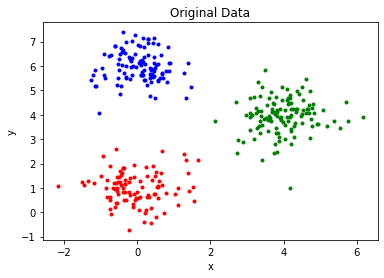
\includegraphics[width=0.8\textwidth]{Original_Data.png}
    }
\end{figure}
\section{实验结果分析}
\subsection{K-Means混合聚类测试结果}
使用K-Means聚类算法的分类结果如下:
\begin{figure}[H]
    \centering
    \subfigure[K-Means聚类算法结果]{
    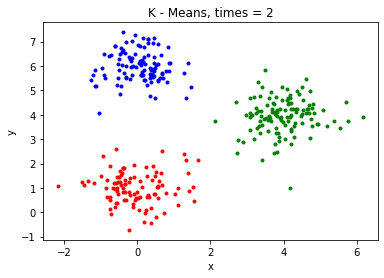
\includegraphics[width=0.8\textwidth]{K-Means_Ans.png}
    }
\end{figure}
我们可以看出分类的情况较好,明显将三类数据分离开来。且迭代次数也较少,仅仅通过两次迭代就得出了结果。
\subsection{高斯混合聚类测试结果}
使用高斯混合聚类的分类结果如下:
\begin{figure}[H]
    \centering
    \subfigure[高斯混合聚类测试结果]{
    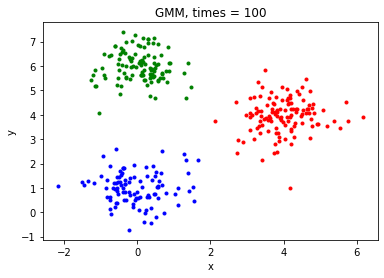
\includegraphics[width=0.8\textwidth]{GMM_Ans.png}
    }
\end{figure}
此处的分类结果也与实际情况较为符合。
\subsection{UCI数据集测试结果}
我们继续使用Lab2中的数据集进行聚类测试,在高斯混合聚类的方法下迭代50次后,分类效果较为良好,准确率如下:
\begin{figure}[H]
    \centering
    \subfigure[UCI数据集测试的准确率]{
    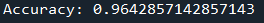
\includegraphics[width=0.8\textwidth]{UCI.png}
    }
\end{figure}
但实际上,可能由于给数据集的特征并不分布并不明显,导致其聚类后准确率在部分情况下接近于0.5。
\section{结论}
\subsection{聚类结果与初始均值选取的关系}
在实验过程中,我以完全随机的方式选择初始点,在实际运行的过程中,发现聚类结果与初始点的选择有着较大的关系,若初始点选择较为失败,会导致聚类效果与实际偏离较大,如下:
\begin{figure}[H]
    \centering
    \subfigure[原始数据]{
    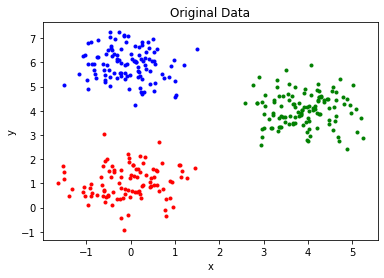
\includegraphics[width=0.4\textwidth]{w1.png}
    }
    \subfigure[K-Means聚类结果]{
    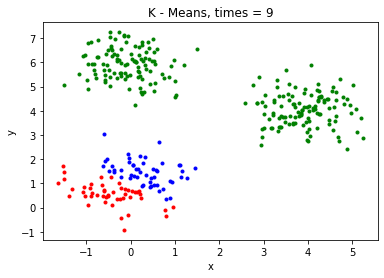
\includegraphics[width=0.4\textwidth]{w2.png}
    }
\end{figure}
可以明显看出,在初始点选择较为失败的情况下,会使聚类陷入局部最优解,导致聚类的效果不太理想。\par
在此提出一种启发式的选取初始点的方法,即我们首先随机选取一个点,每次都在剩余数据集合中选出距离该点最远的一个点,这样能够选出更适合优化进行的初始点集。\par
\subsection{两种聚类方法对比}
K-Means聚类算法是直接在原型数据的基础上进行优化,原理和思路较为简单,但当初始点集选择不好时,可能会陷入局部最优解导致聚类效果不理想。\par
高斯混合聚类是采用概率模型,根据数据集通过多次迭代优化参数,再根据每个数据的分布情况选出其最有可能属于的类别,簇划分由原型对应的后验概率决定。
\end{document}